
% !TEX root = DesignDocument.tex

\chapter{Design  and Implementation}

\section{Systems Goals}
\begin{itemize}
	\item Provide an easy-to-use 2D simulation environment
	\item Simulate realistic physics as best as possible
	\item Allow for easy modification and extension of the simulation
	\item Allow for saving simulations to be re-loaded at a later time
	\item Allow for design of custom robots to use in the simulation
\end{itemize}

\section{System Overview and Description}
There are six major components in this system
\begin{itemize}
	\item Application core
	\item Genera User Interface
	\item World Visualization
	\item Physics Engine
	\item File Read/Write
	\item Plugin System
\end{itemize}
See figure \ref{fig:systemdiagram} for an overview representation of where the components reside in the application and what other components they connect to.

\begin{figure}[tbh]
\begin{center}
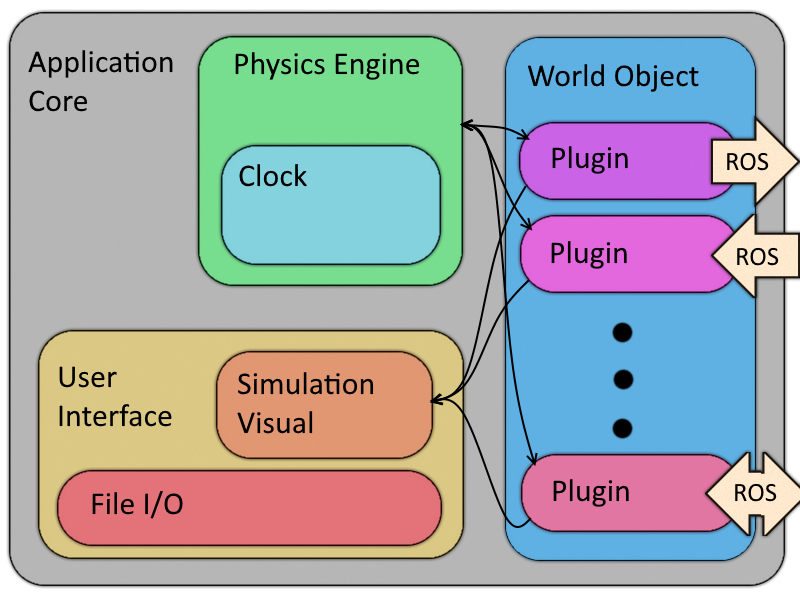
\includegraphics[width=0.75\textwidth]{./images_design/sysarch}
\end{center}
\caption{A visual representation of the system architecture, including basic data paths\label{fig:systemdiagram}}
\end{figure}

\subsection{Application Core}
The Application Core has the job of organizing the rest of the system. It connects all of the events generated by the other components and keeps track of all simulated objects. It is also responsible for adding and removing simulated objects when commanded to.

Explained in more detail below, anything simulated in the application can be represented in the World Object class. The World Object exposes functions to
\begin{itemize}
	\item Add/Remove itself from the physics engine
	\item Obtain its Models for drawing on screen
	\item Obtain its list of Properties
\end{itemize}

Models and Properties are fully defined below as well.

\subsection{Physics Engine}
The Physics Engine is the backbone of the simulation. The main purposes of the Physics Engine are
	\begin{itemize}
		\item Track what objects are part of the simulated world
		\item Step the simulated world at a regular rate
		\item Notify simulated objects when the world updates
	\end{itemize}
Forces can be applied to the simulated objects at any point in time, by any part of the application. The Physics Engine does not concern itself with where the forces originate, just the effects of them.
 
\subsection{User Interface}
The User Interface consists of all portions of the UI which are not the visualization of what is actually being simulated. The UI is responsible for things like providing the user with ways to load and save files, start and stop the simulation, and edit the properties of the simulated objects.

While the visualization of the of the simulated activity is, technically speaking, part of the UI, it is accessed through a UI and thus can be developed independently and the UI general is agnostic to how it looks and behaves. We will reference the visualization in this document in terns such "World Visual", or "Visualization Widget".

\subsection{World Visualization}
The World Visualization is a widget in the UI which is responsible for portraying the simulated activity. Its communication is strictly with the general UI, as it is a child object of it. The UI is expected to tell this visual when objects are added and removed, as well as what models belong with those objects.

\subsection{File Read/Write}
The File Read/Write component is utilized by the general UI. When the user selects a file, the Read/Write component loads or save a world object or collection of world objects in that file. If the file is malformed, it returns an error that the UI can display.

\subsection{Plugin System}
The Plugin System keeps the core application logic separate from the specific capabilities of the simulated objects. Plugins provide the components which make up the objects simulated. Using this design allows users to write their own components for the simulation if some desired feature is missing.

\section{Technologies Overview}
\subsection{C++}
	The entire application is written using the C++ programming language. Reference material for the syntax and libraries provided as part of the language can be found at \url{http://en.cppreference.com/w/}. The most recent standard used by this project is C++11.
	
\subsection{Qt}
	Qt is a cross-platform development framework and library. It is utilized in this project for a couple of its specific features
	\begin{itemize}
		\item Event Loop
		\item QObjects
		\item Signals and Slots
		\item Plugins
		\item Widgets Library
		\item Graphics Framework
	\end{itemize}
	Information about the project can be found at \url{http://doc.qt.io/}. Some of the core concepts of these features are describe in the following sections.
	
	An example containing QObjects and Signals and Slots can be seen in listing \ref{lst:qobjexample} below.
	
\subsubsection{Event Loop}
	The central part of Qt is the Event Loop. When a Qt application is started, it generally enters an event loop which spins during idle time. When an event happens, it is queued until the start of the next iteration of the event loop. Each iteration of the event loop, all pending events are delivered to their receivers to be handled.
	
	\begin{lstlisting}[caption={Pseudocode for the Qt Event Loop}]
while(application_running)
{
	for(event in event_queue)
		handleEvent(event)
	Remove handled events
}
	\end{lstlisting}
	
	Many events are user-generated by actions such as clicking buttons, typing text, and resizing windows. Other events may take the form of cross-thread communication through Signals and Slots.
	
\subsubsection{QObject}
	QObjects are the base type of anything residing in the Qt event framework. Similarly to how all Java types inherit Object, all Qt objects inherit QObject. There are two parts to QObject inheritance.
	\begin{enumerate}
		\item Inheriting QObject will add a number of common functions, signals, and slots to a type. When QObjects are instantiated, they can be given a parent QObject. When a parent QObject is destroyed, it will automatically destroy all of its children.
		\item The Q\_OBJECT macro must be placed in the \lstinline|private| portion of the class definition. At compile time, the Qt Meta Object Compiler (or MOC) is run before the standard C++ compiler. The MOC finds this macro and other Qt-specific keywords and generates standard C++ files which a normal compiler, such as g++, can use.
	\end{enumerate}
	
	Limitations on inheritance of QObject
\begin{enumerate}
	\item QObject cannot be inherited in a templated class
	\item If multiple types are inherited, QObject (or a type that isa QObject) must be the last type inherited
	\item QObject cannot be virtually inherited, so the diamond inheritance problem cannot be resolved if all types are QObjects
\end{enumerate}
	
\subsubsection{Signals and Slots}
Signals and Slots allow programmers to define custom events and event handlers in their objects. 

A Signal is a public method of a QObject which has no definition. (The definition is added by the MOC). Instantiated QObjects can emit signals at any point in time. Signals may have parameters, and when the object emits a signal with parameters, it will fill them with data.

A Slot is a public, protected, or private method of a QObject. It must have a full definition just like any other method. (In many cases, it can be treated exactly as if it were a regular method.)

There are two main limitations on Signals and Slots
\begin{enumerate}
	\item All parameters MUST be pass-by-value. This allows all data to be copied, preventing race conditions when signals trigger slots in other threads.
	\item Custom types passed as parameters in signals and slots must be known to the Qt Meta-Object System. See documentation on the qRegisterMetaType() function for more information on how this works.
\end{enumerate}

At runtime, applications can connect the signals of instantiated QObjects to the slots of any other instantiated QObjects. When a QObject emits a signal, any slots that it is connected to will be called.


\begin{lstlisting}[language=C++, caption={Example of QObjects with parenting, Signals and Slots, and connections.\label{lst:qobjexample}}]
class foo : public QObject
{
	Q_OBJECT
public:
	//Construct with optional parent QObject
	foo(QObject* parent=nullptr) : QObject(parent){}

//Keyword known to MOC
//All signals are public methods
signals:
	void somethingHappened();
	void otherThingHappened(int);

//Another MOC keyword. Slots can be public, private, or protected
public slots:
	void reactToAnotherThing(int x)
	{
		cout << "Another thing: " << x << endl;
	}
};

class bar : public QObject
{
	Q_OBJECT
public:
	//Construct with optional parent QObject
	bar(foo* parent) : QObject(parent)
	{
		//Connect events between objects
		//Note that events and handlers have the same function signature	
		
		//When somethingHappened() is emitted by 'parent'
		//Do reactToSomething() in 'this'
		connect(parent, &foo::somethingHappened,
		        this, &bar::reactToSomething);
		
		//When otherThingHappened() is emitted by 'parent'
		//Do reactToOtherThing() in 'this'
		connect(parent, &foo::otherThingHappened,
		        this, &bar::reactToOtherThing);
		
		//When anotherThingHappened() is emitted by 'this'
		//Do reactToAnotherThing() in 'parent'
		connect(this, &bar::anotherThingHappened,
                parent, &foo::reactToAnotherThing);
	}

//Keyword known to MOC
//All signals are public methods
signals:
	void anotherThingHappened(int);	

//Another MOC keyword. Slots can be public, private, or protected
private slots:
	void reactToSomething()
	{
		cout << "Something happened!" << endl;
	}
	
	void reactToOtherThing(int x)
	{
		cout << "Reacting to other thing: " << x << endl;
		
		//Send a signal back to 'parent' object
		emit anotherThingHappened(x+1);
	}
};

int main()
{
	//Put a 'bar' on the
	foo* f = new foo();
	bar* b = new bar(f);
	
	//This will delete b as well because 
	//b is a child of f
	delete f;
}
\end{lstlisting}

\subsection{Box2D Physics}
The Box2D library is used as the basis of the Physics Engine for this simulation. It is a C++ library which can be used for realistic physics simulation and collision detection. The Box2D project is hosted on github at this location \url{https://github.com/erincatto/Box2D}.

When working with a Box2D simulation, there are a number of types that are used.
\begin{itemize}
	\item b2World: Container for everything being simulated and all extra simulation information. Bodies and Joints are added directly to the World to be simulated.
	\item b2Body: Container for physics information for one specific element of the simulation. Bodies are made up of any number of Fixtures, which are held relative to each other as the body moves. Bodies contain information such as mass, inertia, velocity, etc. Bodies can also be acted upon by forces or impulses.
	\item b2Fixture: Fixtures are used to attach shapes to a Body. Each fixture is used to attach a single shape.
	\item b2Shape: Abstract base type of any shape. Various shapes are supported by Box2D, but this project utilizes mainly b2PolygonShape and b2CircleShape.
	\item b2Joint: Joints are used to constrain how bodies move relative to each other. Many types of joints exist in Box2D, some examples are rigid, revolute, prismatic, and motor.
\end{itemize}

\subsection{ROS}
As mentioned a number of times previously, this simulation supports communication with external applications through ROS, the Robotics Operating System. Information on ROS can be found at \url{http://www.ros.org/}. The version of ROS targeted for this project is ROS Kinetic Kame.

The core application itself has minimum communication through ROS, it mainly starts a ROS listener thread so that messages can be received. The bulk of the message sending and receiving is done by the plugin components which make up the objects being simulated.

 \section{Architecture and System Design}
 	The simulation underwent a number of design changes during its development. This section will detail designs which were discussed, removed, or otherwise not used as well as the design concepts, datatypes, and flow of the final product.
 	
 \subsection{Design Selection}
 \subsubsection{UI}
 	When building a cross-platform user interface in C++, there are only a few options available. When discussing this, the following ideas were brought up: Pure OpenGL, Qt QML, and Qt Widgets. The final decision was Qt Widgets, which will be discussed below.
 	
 	A pure OpenGL solution was not selected due mainly due to the difficulty of implementation and the amount of work that would have to go into a UI of that nature. If using Qt were not an option, pure OpenGL may have been selected; however, having the Qt library available makes it hard to justify the amount of extra development that a pure OpenGL solution would add.
 	
 	When writing a UI in Qt, there are two main options for the core library: Widgets and QML. Qt Widgets has been around longer and is generally used to produce applications that look and feel 'like a desktop program'. The Widgets library contains many commonly used pieces which can be organized into a UI, similarly to how C\# Forms or Java Swing works. Qt QML is a newer library which is being actively developed with Qt. QML separates the UI entirely from the business logic by running the UI in a custom javascript interpreter. The main advantages to QML are that it's very easy to develop QML UIs without any business logic and it's currently receiving the bulk of support in new versions of Qt. QML would have been the first choice for the project UI, but it is difficult to use on an fresh system. Widgets projects require just a set of shared objects to run, but QML projects require a number of shared objects as well as some basic QML code files which are parsed at runtime. These additional files are not usually present in the base library installation of Qt, so using QML would have meant that the end user would need to resolve extra dependencies to run the application.
 	
 	\subsubsection{World Visualization}
 	Within the Qt Widgets library, there are a number of different ways build a widget with a drawing canvas that shapes can be shown on. The most primitive method is to create an OpenGL drawing window which is contained in the widget. The other main option is to use the Qt Graphics Framework, which is an abstraction layer for drawing 2D objects on a background with OpenGL.
 	
 	Again, it was decided that the pure OpenGL solution would ad unnecessary development time, and an alternative should be used. Not only does the graphics framework provide easy methods for drawing primitive shapes on a canvas, but it also allows for parent-child relationships between the models, which in turn allows shapes to be defined with relative transforms to each other instead of everything needing to be in world coordinates.
 	
 	\subsubsection{Physics}
 	One of the main failings of STDR was its lack of a physics engine. It was decided early on that a known physics engine should be used, or one should be written for this project so that at least basic collision detection could be simulated.
 	
 	A number of different engines were investigated, including Box2D and Chipmunk2D. In the end, Box2D was chosen because it is simple and lightweight while also providing all of the functionality necessary for this simulator. Other physics engines would have been too bulky or difficult to use, and writing a custom physics engine would have extended the development considerably and likely would have resulted in worse performance.
 
 %\subsection{Data Structures and Algorithms}
 
 %\subsubsection{Importing Images}

 %TBD 
 
 \subsection{Data Flow}
 All data flows between the major system components through Qt Signals and Slots. There are four main events which drive data flow
 \begin{itemize}
 	\item World Object Added
 	\item World Object Removed
 	\item Simulation Ticked
 	\item Plugin Receives External Input
 \end{itemize}
 
 \subsubsection{World Object Added}
 	World Object additions are generally initiated by the UI. When the user wants to add an Object to the simulation, the UI signals to the core indicating what Object should be added. The core copies the World Object and stores the copy with an index. The Object and its index are sent back to the UI and Physics engine wrapped in interfaces which can be used to access methods of the new World Object. More information on these interfaces can be found in the World Object class details below.
 	
 	When the Physics engine receives a new World Object, it passes the b2World object
of the simulation to it so that the Object can add bodies and shapes to the physics engine.

	When the UI receives a new World Object, it passes the object's Model to the world view to be drawn and caches the list of object Properties. When the user selects this Object, those Properties are displayed for viewing and editing.
	
 \subsubsection{World Object Removed}
 The process of removing a World Object is very similar to that of creating one. The UI signals to the core that the user would like to remove an Object; this Object is identified by the index that was assigned when it was added to the simulation. The core then signals back to the UI and Physics that this Object is removed and deletes the associated Object from the heap.
 
 When the Physics engine receives this signal, it passes the b2World to the Object again so that the Object can remove any Box2D bodies and joints that it created.
 
 When the UI receives this signal, it un-caches the Object's list of Properties and notifies the world view widget to stop drawing the Models associated with the object.
 
 \subsubsection{World Ticked}
 World ticks are generated by the physics engine on a timer. The default tick rate is 100 per second, and each tick moves the simulation forward $\frac{1}{100}$ of a second.
 
 When the world tick signal is received by a World Object, it checks the location of its Box2D body, and, if it moved, updates its Model, causing a redraw in the world view widget. Likewise, when a Component of an Object receives this signal, it may also update its own Model. Additionally, Components can take this moment to modify the simulation by applying forces on their Box2D bodies.
 
 \subsubsection{External Communication}
 The most common example of external communication is robot control code signaling that wheel velocities should change. When World Object Components receive an external communication of this nature, they can apply forces on their associated Box2D body to affect the simulation. This change will be applied on the next tick to happen after the force is applied.
 
  \subsection{Interfaces}
  \subsubsection{Physics Engine Interface}
  The SimulationPhysics\_If interface (UML Figure \ref{uml:phys_if}) provides the interface any Physics Engine used in this simulation must follow. It is expected that any Physics Engine will be built on Box2D.
  
  There are four main methods for modifying the flow of the simulation and two main methods for influencing what is actually simulated.
  
  The methods for changing simulation flow are
  \begin{itemize}
  	\item start()
  	\item stop()
  	\item clear()
  	\item setTick()
  \end{itemize}
  
  The methods for adding and removing simulated objects are
  \begin{itemize}
  	\item addWorldObject()
  	\item removeWorldObject()
  \end{itemize}
  The WorldObjectPhysics type passed to the addWorldObject function is explained in conjunction to the World Object in section \ref{sec:worldobjclass}.
  
  The Physics Engine should emit the following signals under appropriate circumstances.
  \begin{itemize}
  	\item physicsStarted()
  	\item physicsStopped()
  	\item physicsTickSet()
  \end{itemize}
  
  \subsubsection{UI Interface}
  
  \subsubsection{View Widget Interface}
  
  \subsubsection{File Handler Interface}
  
  \subsubsection{World Object Component Interface}
  
  \subsubsection{World Object Component Plugin Interface}

 \subsection{Classes}
  \subsubsection{Model}
  The Model class is a container for shapes; it is designed to be used communicate what should be drawn on the screen. When models change or move, signals are emitted so that the image drawn can update to reflect the changes.
  
 	The UML of the Model class is in UML Figure \ref{uml:model}. The Model class provides constructors to initialize it with any number of children or shapes, and exposes get() functions for both. After construction, shapes and children models can be added and removed with the four functions
 \begin{itemize}
 	\item addChildren()
 	\item removeChildren()
 	\item addShapes()
 	\item removeShapes()
 \end{itemize}
 Calling any of these functions will result in the modelChanged() signal being emitted. If a child model emits modelChanged(), then the parent will forward that call with the childModelChanged() signal. This design allows the UI to recalculate shapes only when necessary, instead of every frame.
 
 The transform of the model can be accessed through getTransform() and setTransform(). Setting the transform will result in the transformChanged() signal being emitted, and similarly to how the modelChanged() signals work, the parent of a model whose transform changes will forward that signal with childTransformChanged().
 
 All children of a Model should exist on the heap. Upon its deletion, the Model will delete all of its children. The shapes of a Model may exist anywhere in memory, as the Model will NOT delete its shapes at any time.
 	
 \subsubsection{Property}
 	Properties are variables within an object that may be modified by external sources. They are accessed through PropertyView objects, which enforce read/write rules so that internal state that should not be changed is not changed by accident. The UML for Properties, PropertyViews, and all associated types is found in UML Figure \ref{uml:property}
 	
 	A Property has three main parts
 	\begin{itemize}
 		\item Its PropertyInfo
 		\item A validation function
 		\item Its value
 	\end{itemize}
 	
 	The PropertyInfo is a container for any meta information about the Property. This contains data such as the type of the data, whether or not it's read-only, whether or not it's a list, and a description of what the Property is used for. This is intended to be used to aid UI which displays Properties to the user. It is assigned to a Property once, at construction, and can be accessed by the info() method.
 	
 	The validation function follows the prototype \lstinline|function<QVariant(QVariant, QVariant)>| and is used to make sure that the data assigned to the Property is valid. The first parameter represents the previous value, and the second parameter is a potential new value. The function should return the new value if it is acceptable and the old value if the new one is not acceptable. By default, this function accepts all values. A number of basic validation functions exist as static members of the Property class. Some of them are
 	\begin{itemize}
 		\item double\_validator()
 		\item int\_validator()
 	\end{itemize}
 	
 	The value of a property is accessed and mutated though the methods set() and get(). get() returns the current value. set() validates a new value using the validation function and stores whatever value is returned. Whenever the set() function is called, the valueSet() signal is emitted.
 	
 	The internal slot \_set() receives signals from PropertyView objects when they want to change the value stored in the Property. It behaves similarly to the set() function.
 	
 	The internal slot \_update() is used to re-publish the value to all PropertyView objects which are watching the Property.
 	
 	The PropertyView object contains all of the same public functions as a Property; however it is constructed with only a Property, which it observes. When the set() function is called on a PropertyView, the requestValue() signal is emitted, and original Property handles that signal and validates the new value. The valueSet() signal in a PropertyView is tied to the same signal in its observed property so that any owner of a PropertyView will know when the value changes.
 	
 	The internal slot \_invalidate() is called with the observed Property is destroyed to prevent a null reference. If any accessors are called after this happens, they will return default-constructed values. It is intended that the owner of a PropertyView will receive some indication that the PropertyView should no longer be tracked from another source.
 	
  \subsubsection{World Objects} \label{sec:worldobjclass}
	The main data type in this simulation is the World Object. World Objects can be added to and removed from the simulation, cloned, and saved to or loaded from files. World Objects consist of a set of Components (Which follow the WorldObjectComponent\_If interface and are created by plugins) and the constraints that keep them together. For the UML diagram of a World Object, see Figure \ref{uml:worldobj}.
	
	World Objects, upon construction, consolidate all of the models and properties of its components. When getModels() or getProperties() is used to access the World Object, these consolidated lists are returned.
	
	It is possible that some of a World Object's components will use external communications, such as ROS. The usesChannels() accessor is used to determine if this is the case, and the connectChannels() and disconnectChannels() slots are used to start or stop communctions of any components which do this.
	
	Only the Simulator Core holds the reference to a World Object in the simulation. As can be seen in the UML diagram, a number of wrapper objects exist to provide specific interfaces. The WorldObjectProperties class provides an interface to a World Object which is used by the User Interface, and the WorldObjectPhysics provides the interface used by the Physics Engine. These interfaces are children (in the Qt sense) of the original World Object, so no owner of an interface needs to delete their interface when the WorldObject is removed from the simulation.
	
	When a World Object is added to the physics engine, it should be given access to the Box2D world. At this point, the World Object and its Components create any Box2D bodies needed and set up the shapes, masses, and joints required to simulate the World Object. During the simulation, Components can apply forces to this body to give motion to the World Object. When the World Object is removed from the physics engine it should be given access to the Box2D world again so that all bodies and joints can be removed from the simulation. These two events are the only points in time that the World Object will add or removed elements of the simulated world.
 
 \subsection{UML}
 \begin{figure}
 	\begin{center}
 	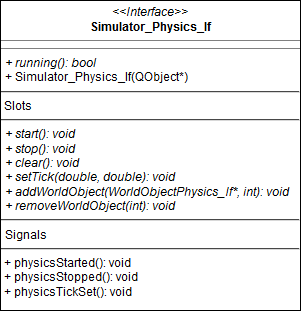
\includegraphics[scale=0.5]{./images_design/uml/Physics_Engine_If}
 	\caption{UML of Physics Engine class interface\label{uml:phys_if}}
 	\end{center}
 \end{figure}
 
  \begin{figure}
 	\begin{center}
 	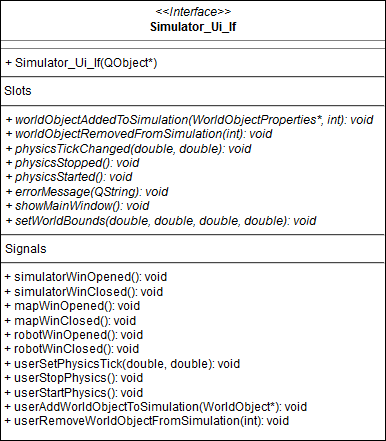
\includegraphics[scale=0.5]{./images_design/uml/Ui_If}
 	\caption{UML of UI class interface\label{uml:ui_if}}
 	\end{center}
 \end{figure}
 
  \begin{figure}
 	\begin{center}
 	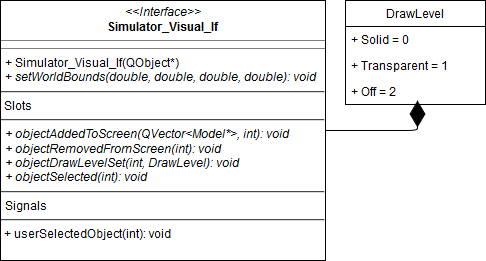
\includegraphics[scale=0.5]{./images_design/uml/Visual_If}
 	\caption{UML of Visualization widget interface\label{uml:visual_if}}
 	\end{center}
 \end{figure}
 
 \begin{figure}
 	\begin{center}
 	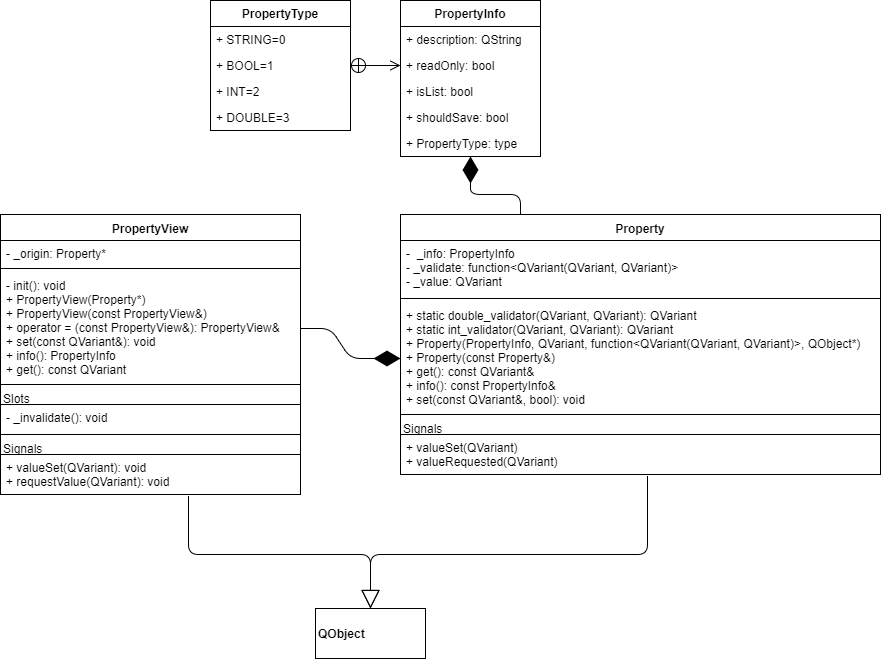
\includegraphics[scale=0.5]{./images_design/uml/Property}
 	\caption{UML of Property and associated classes\label{uml:property}}
 	\end{center}
 \end{figure} 
 
 \begin{figure}
 	\begin{center}
 	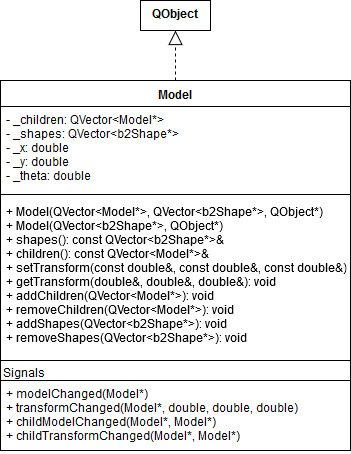
\includegraphics[scale=0.5]{./images_design/uml/Model}
 	\caption{UML of Model\label{uml:model}}
 	\end{center}
 \end{figure} 
 
  \begin{figure}
 	\begin{center}
 	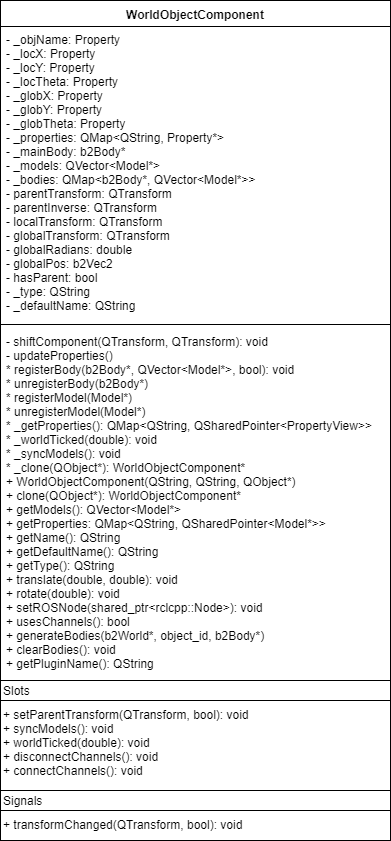
\includegraphics[scale=0.5]{./images_design/uml/WorldComponent_If}
 	\caption{UML of World Component class interface\label{uml:worldcomponent_if}}
 	\end{center}
 \end{figure} 
 
   \begin{figure}
 	\begin{center}
 	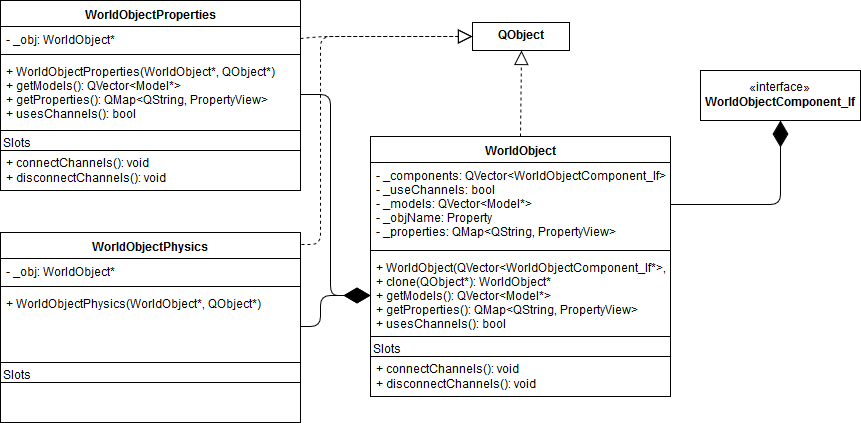
\includegraphics[scale=0.5]{./images_design/uml/WorldObj}
 	\caption{UML of World Object and associated classes\label{uml:worldobj}}
 	\end{center}
 \end{figure}
 
 \begin{figure}
 	\begin{center}
 	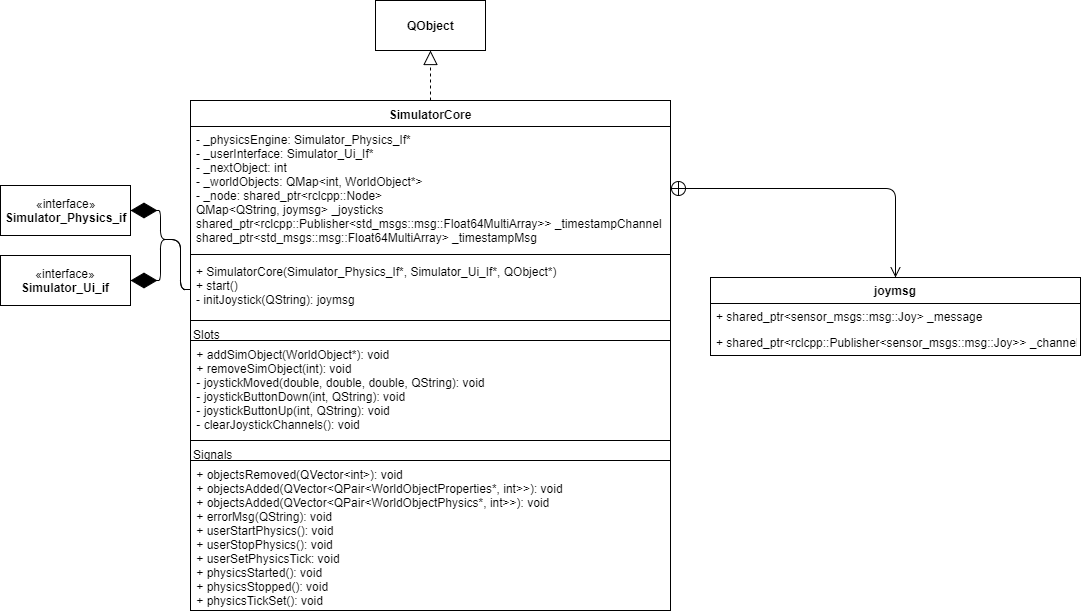
\includegraphics[scale=0.5]{./images_design/uml/SimCore}
 	\caption{UML of Simulator Core\label{uml:simcore}}
 	\end{center}
 \end{figure}
 
 \begin{figure}
 	\begin{center}
 	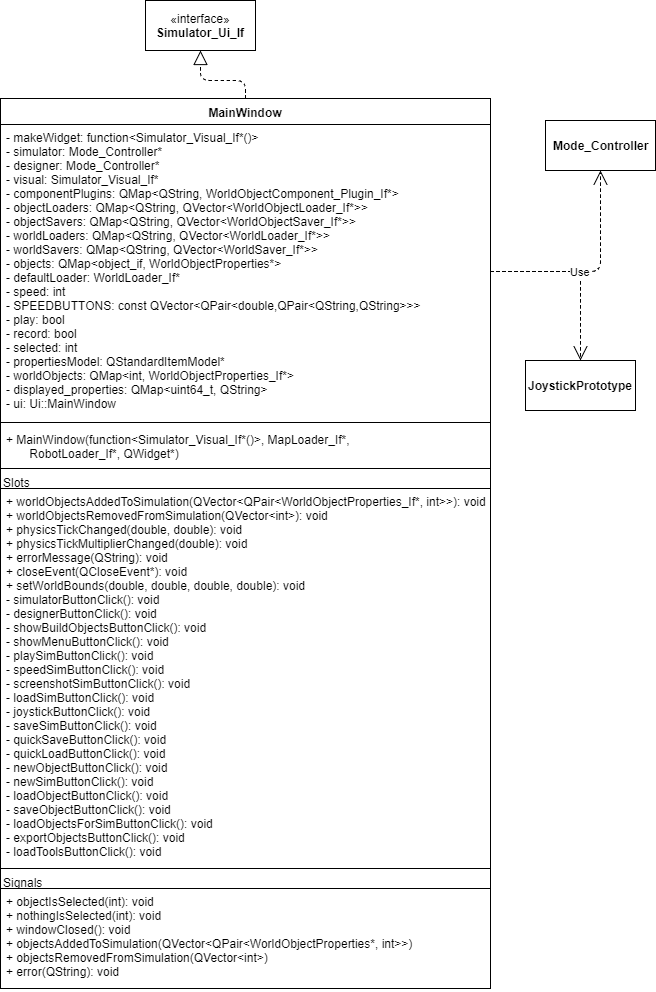
\includegraphics[scale=0.5]{./images_design/uml/MainWindow}
 	\caption{UML of User Interface\label{uml:mainwin}}
 	\end{center}
 \end{figure}
 
 \begin{figure}
 	\begin{center}
 	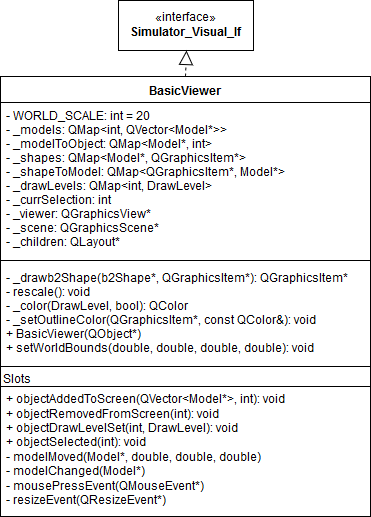
\includegraphics[scale=0.5]{./images_design/uml/BasicViewer}
 	\caption{UML of Visualization widget\label{uml:viewwidget}}
 	\end{center}
 \end{figure}
 
 \begin{figure}
 	\begin{center}
 	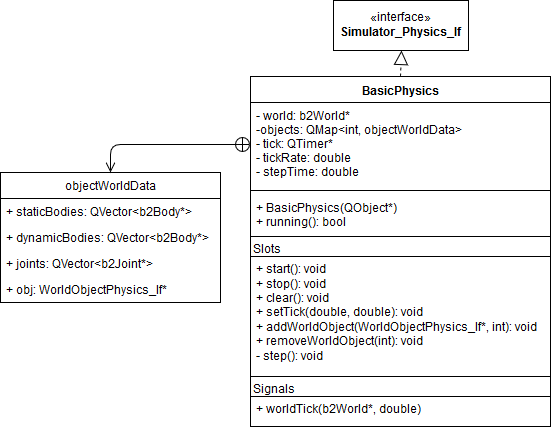
\includegraphics[scale=0.5]{./images_design/uml/BasicPhysics}
 	\caption{UML of Physics Engine\label{uml:physics}}
 	\end{center}
 \end{figure}
 
 \begin{figure}
 	\begin{center}
 	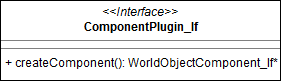
\includegraphics[scale=0.5]{./images_design/uml/ComponentPlugin}
 	\caption{UML of Plugin interface\label{uml:componentplugin}}
 	\end{center}
 \end{figure} 
 
 \begin{figure}
 	\begin{center}
 	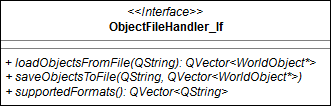
\includegraphics[scale=0.5]{./images_design/uml/FileHandler_If}
 	\caption{UML of File Handler interface\label{uml:filehandle_if}}
 	\end{center}
 \end{figure} 
 
 \subsection{UX}
 
 \subsection{UI}

\section{Simulator Core}

\subsection{Technologies  Used}

\subsection{Component  Overview}
The simulator core is, as the name suggests, the main piece of the simulation. It organizes and marshals the other parts of the system and ensures that data flows in the correct paths. The main purpose of the simulator core is to connect the UI to the Physics engine and keep them synchronized so that what's shown on screen reflects what's simulated in the physics engine. See UML Figure \ref{uml:simcore} for a list of data members and functions in the simulator core.

\subsection{Data Flow Diagram}

 \begin{figure}
 	\begin{center}
 	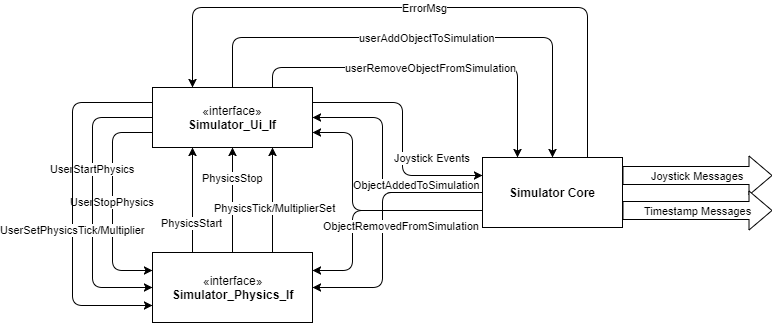
\includegraphics[scale=0.5]{./images_design/uml/DataFlow_simcore}
 	\caption{Data Flow in Simulator Core\label{uml:dataflow_simcore}}
 	\end{center}
 \end{figure} 

\subsection{Design Details}

\section{Physics Engine}

\subsection{Technologies  Used}
\begin{itemize}
	\item Qt
	\item Box2D
\end{itemize}

\subsection{Component  Overview}
The physics engine is responsible for updating the world state at regular intervals. When objects are first added to the world, they should be initialized in the physics engine, and until they are removed from the world they should be simulated along with the rest of the objects. The physics engine should be capable of starting, stopping, changing rate, and adding or removing an object while in any state. The current physics engine is the 'BasicPhysics' object found in UML Figure \ref{uml:physics}. The interface that it follows is found in UML Figure \ref{uml:phys_if}

\subsection{Data Flow Diagram}

 \begin{figure}
 	\begin{center}
 	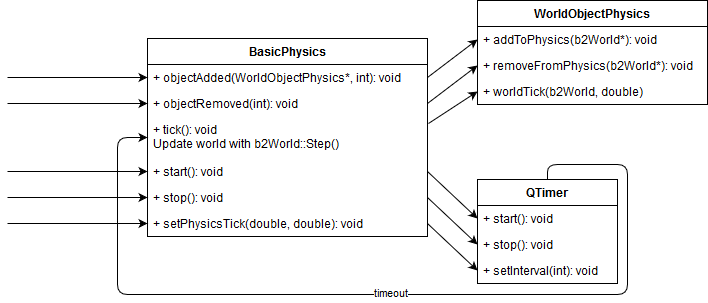
\includegraphics[scale=0.5]{./images_design/uml/DataFlow_physics}
 	\caption{Data Flow in Physics Engine\label{uml:dataflow_physics}}
 	\end{center}
 \end{figure}

\subsection{Design Details}


\section{Major Component \#3 }

\subsection{Technologies  Used}
This section provides a list of technologies used for this component.  The details 
for the technologies have already been provided in the Overview section. 

\subsection{Component  Overview}
This section can take the form of a list of features. 

\subsection{Phase Overview}
This is an extension of the Phase Overview above, but specific to this component. 
 It is meant to be basically a brief list with space for marking the phase status. 

\subsection{ Architecture  Diagram}
It is important to build and maintain an architecture diagram.  However, it may 
be that a component is best described visually with a data flow diagram. 


\subsection{Data Flow Diagram}
It is important to build and maintain a data flow diagram.  However, it may be 
that a component is best described visually with an architecture diagram. 


\subsection{Design Details}
This is where the details are presented and may contain subsections. 


